\chapter{Часть 3}
\section{Египетские контрасты}

В этой части мы немного отвлечёмся от воздушных сражений (окей, и компенсируем это в последней, четвертой части), и немного поговорим о том, как вообще советские люди, внезапно оказавшиеся в тысячах километров от дома, на другом континенте, в другом климате и другой культуре, эту самую другую культуру видели.

От переводчиков и технарей — до послов и генералов. Из кабинетов резиденции Главного военного советника, куда почти не долетал грохот разрывов снарядов — и из «мальги» на Суэцком канале, где этот грохот рождали израильские бомбы. Так получилось, что «Египет» у каждого из них был свой. Одни видели яркие витрины магазинов, другие - пустыню, до горизонта. Видели его таким разным.

Униженным «неделей израильского военного искусства» в 67-м, затянутым светомаскировкой. И — весёлым и беззаботным, с ночными клубами и вечеринками, так похожий на таинственный Запад. Сияющим, как Солнце, заходящее за вечные пирамиды Гизы. И нищим, как жестокие феллахи, каждый день, как и их предки тысячу лет назад, начинающие свой скорбный путь, обреченные от рождения до смерти видеть бесконечные поля дельты Нила.

Или — умереть на алтаре великих амбиций египетских правителей.

Когда-то, столетия назад, египетские фараоны строили себе гробницы, призванные стать величайшим чудом на земле и оставить в веках величие погребенных под ними людей. Так, ценой тысяч жизней ввысь устремились величайшие чудеса Античности — Пирамиды Гизы. Теперь потомки этих крестьян погибали на другой великой стройке. В этот раз они зарывались вглубь земли, там, где через несколько недель вознесутся к небу острыми и хищными носами боги войны нового времени, призванные защищать землю фараонов. А с неба на строителей охотились сошедшие с барельефов древних доисламских храмов птицы. Пикируя к земле, и возвращаясь на небо, оставляя за собой разбитые куклы, некогда бывшие египетскими строителями-феллахами. И так — каждый раз, когда ладья Ра поднималась по небесной реке. Страшные птицы с острой шестиконечной звездой на крыльях приносили новые могилы на кладбищах, внезапно окруживших великие стройки того, кто решил назвать себя наследником древних Фараонов ...

\section{Люди пустыни}

Большинство простых советских людей из 18-й зенитно-ракетной дивизии о пирамидах читали разве что в курсе истории древнего мира. Тем более удивительным для них становилось соприкосновение с миром современным. А он терял свой волшебный флёр древности довольно быстро. Первым, что встретило советских солдат, была страшная выматывающая жара. Из привычных Нижнего Новгорода, Николаева, и даже Ашулука, они отправились в настоящую пустыню.

Вспоминают советские военнослужащие:
\begin{textcitation}
	Чтобы постоянно быть в физической форме, летчик должен заниматься физкультурой. В условиях Северной Африки, когда температура доходила до +49 °C в тени, организованных занятий физкультурой не проводилось, но практически все занимались по личному плану. На скамейке качали пресс, гантелями и эспандерами поддерживали тонус организма, скакали через веревочку как дети. Я в числе немногих бегал, считая, что это лучший способ тренировать выносливость, нагружать сердечно-сосудистую систему. Бог мой, как это монотонно, просто насилие! 
\end{textcitation}

В.Б.Ельчанинов (лётчик 135 истребительного авиаполка)
\begin{textcitation}
	Поэтому дежурство стало изнурительным, тем более что температура воздуха доходила порой до +50 градусов, на станциях наведения ракет, радиолокационных станциях в отдельные дни температура достигала +60 градусов. Донимали нас и песчаные бури, которые загоняли мельчайший песок повсюду: в аппаратуру, приборы, технику, продукты и т. д.
\end{textcitation}
Б.И. Жайворонок (подполковник, командир 1-й зенитно-ракетной бригады 599-го полка)
\begin{textcitation}
	Даже в тени температура достигала иногда 53 градуса.
\end{textcitation} 

В.В.Захаров (С-125)
\begin{textcitation}
	Напряжение физическое, когда с восхода до захода солнца — утомительное боевое дежурство с готовностью к немедленному пуску ракет при температуре в кабине до 60 градусов. А по ночам — бесконечные, до изнеможения тренировки по свертыванию и развертыванию техники, передислокации. 
\end{textcitation}
А.Я.Костин (начальник политотдела зенитно-ракетной бригады)
\begin{textcitation}
	"Очень хочется зайти в землянку с огнеметом и произвести «дезинфекцию»
\end{textcitation}

Жара сама по себе была проблемой — но, как ни странно, едва ли не наименьшей. В конце концов, служили же в Средней Азии, в Казахстане. Почти к любой жаре можно так или иначе привыкнуть. Проблема была в том, что в пустыне были обитатели, которые изрядно портили жизнь советским солдатам. Речь, как ни странно, не о египтянах — они, как раз, как могли старались помочь устроиться в новых условиях.

\begin{figure}[h!tb] 
	\centering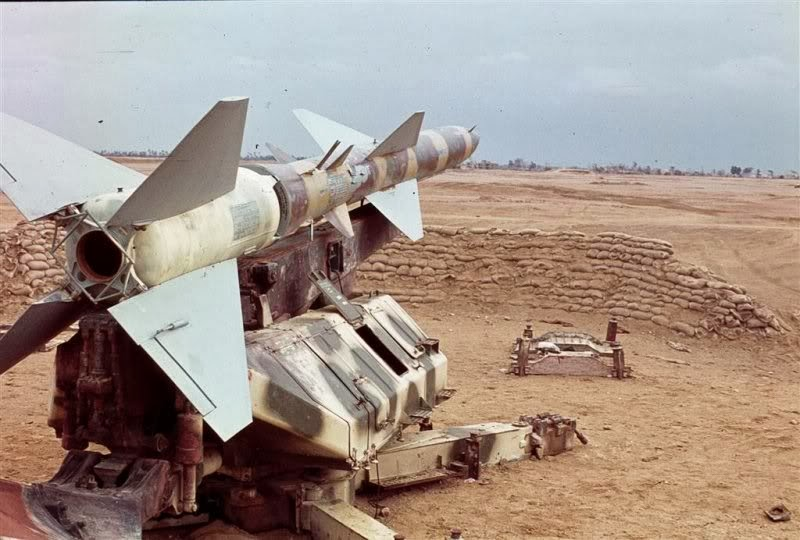
\includegraphics[scale=0.4]{Dolina_2/F8dlw3qe7jg.jpg}
	%	\label{fig:scipion} % Unique label used for referencing the figure in-text\end{document}
	%	%\addcontentsline{toc}{figure}{Figure \ref{fig:placeholder}} % Uncomment to add the figure to the table of contents%----------------------------------------------------------------------------------------
	\caption{Здесь должны быть скорпион и сольпуга, но что-то пошло не так}%	CHAPTER 2
\end{figure}

Пустыня кишила фалангами, скорпионами, змеями. Каждая мальга, каждая траншея для них — укрытие от палящего солнца. Каждый оставленный сапог и ботинок — отличное убежище. Опять же, служившие или родившиеся в Средней Азии солдаты встречались с ними — но не в таких количествах и не в таком объёме. Зачастую встречи с этими тварями происходили совершенно случайно - солдат спросонья надевал на ногу сапог, забыв вытряхнуть оттуда ночного оккупанта, после чего с громким криком, прыгая на одной ноге, сдирал его с себя. Или садился на камень, тревожа его зловредного обитателя.

Укус фаланги, хоть и не был ядовит, был черезвычайно болезненным. Да и часто приводил к сходным последствиям — на её челюстях-хелицерах часто оставались гниющие остатки её предыдущей пищи.

Поначалу, в 18-й дивизии фиксировали 20-30 случаев укусов в день. Нет, серьёзно, от пустынной живности пострадало на порядок больше советских солдат, чем от израильских бомб. Другое дело, что к смертельному исходу такие укусы приводили достаточно редко - всё-таки на дворе была вторая половина 20-го века, а не середина 19-го.

Борьба со скорпионами становилась ежедневным испытанием. Советские солдаты быстро научились каждое утро проверять обувь. Чтобы твари не заползали на кровати, ножки ставились в банки с керосином. Это приводило к другой проблеме - в и без того душных землянках-мальгах стало практически невозможно находиться. Спать в помещении, напрочь пропахшем керосином - то ещё удовольствие. Да и керосин не всегда спасал — отдельные тварюшки ухитрялись падать на кровати с потолка. 

Б.И. Жайворонок (подполковник, командир 1-й зенитно-ракетной бригады 599-го полка):
\begin{textcitation}
	…тарантулы и скорпионы, которые залезали в постель, в обувь, доводили порой до психологических стрессов.
\end{textcitation}

А. Г. Смирнов (Генерал-майор, командир 18-й ЗРД ОН)

\begin{textcitation}
	Нельзя не сказать и о комарах, мухах, тарантулах, скорпионах. В первых числах июля я выехал с небольшой группой офицеров на рекогносцировку для выбора стартовых позиций ЗРДН в районе Исмаилии. В группу входили подполковник Пономарев В.А. и майор Полушин, которых я знал очень хорошо по совместной службе. ... Не успели мы расположиться, как налетели желто-коричневые комары по размерам раз в пять больше «наших». Пришлось прекратить обед и выехать на продолжение рекогносцировки. Однако проехать к предполагаемому месту СП не смогли — машина застряла в песке, и мы пошли пешком. Через 100–150 метров я услышал крик. Обернувшись, увидел падающего майора Полушина… 
	
	Прибыли в арабский госпиталь, располагавшийся в 30 км от места происшествия. В арабском госпитале мест не было, поэтому, не получив никакой помощи, мы выехали в свой госпиталь. Это еще 50–60 км пути.
	
	При въезде в госпиталь майор Полушин опять потерял сознание, и в таком состоянии мы передали его в руки наших врачей.
	
	Позднее начальник госпиталя позвонил мне и передал, что если бы мы опоздали минут на пять, все могло бы кончиться плохо. Что же произошло, ведь комары кусали нас всех, а плохо стало лишь одному. Оказывается, пятью днями раньше Полушина ужалил скорпион (в Асуане). Врачи приняли меры, и все обошлось благополучно. Но достаточно было после этого укуса комара, чтобы организм не выдержал. Начало отказывать сердце.
	
	Впоследствии майор Полушин неоднократно вспоминал об этом. Говорил, что мы спасли ему жизнь, не оставив в арабском госпитале. Возможно, в этом есть доля истины…
\end{textcitation}

Н.В. Александрук (сержант, батарея С-125)
\begin{textcitation}
	Забравшись в землянку-мальгу, установили для освещения аккумуляторные фонари с пусковых установок и принялись готовиться ко сну. Чтобы хоть немного отдохнуть, сняли ботинки и куртки, оружие с ремнем положили под матрас в изголовье так, что получилась подушка. Как только потушили фонари, кажется, миллионы вампиров-комаров набросились на разгоряченные тела. Так что буквально через несколько минут пришлось срочно включать освещение. Но комары, ощутив вкус крови, уже больше не упускали возможности подкормиться. Для защиты пришлось с головой укрываться простыней и не выключать электрофонарь. Таким образом удалось уснуть и кое-как отдохнуть. 
	
	Утром, после ночного промежуточного дрема, проснулись от невыносимого зуда. В местах соприкосновения простыни с телом виднелись огромные кровяные пятна, покрытые снаружи полчищами комаров. Усталость за день и хоть и короткий, но довольно крепкий сон позволили огромным комарам делать массовые укусы через простыню без сопротивления спящего. Наутро почти все после сна появились с опухшими лицами и разодранными до крови местами укусов…
\end{textcitation}
Н.Р.Якушев (техник в 135-м истребительном авиаполку)

\begin{textcitation}
	На военном аэродроме Джанаклис, куда нас привезли из Каира, было около ста советских специалистов, в основном, летчики, техники, механики. Я был закреплен за одним из наших самолетов МИГ-21, обслуживал новейшее по тем временам оружие — ракеты с самонаводящимися тепловыми головками.
	
	Работа была напряженная, особенно когда звено на боевом дежурстве. В течение всех суток должна быть готовность номер один. Летчик в кабине самолета, техник и механики рядом с самолетом готовые в любую секунду обеспечить боевой вылет самолета. Психологически выдержать 24 часа в адском напряжении очень тяжело, еще добавить к этому жару в 50 градусов, постоянную угрозу укуса змеи или скорпиона, а может быть, и фаланги, которыми кишит пустыня.
\end{textcitation}

В.С. Логачев (командир стартового взвода дивизиона С-125)

\begin{textcitation}
	Есть приходилось очень быстро. Если зазевался на 1–2 минуты, то суп покрывался мухами в несколько слоев. Их там несметное количество. Отличие арабской мухи от нашей в том, что она более нахальна, не реагирует на отпугивающие взмахи, то есть избавиться от нее можно только одним способом — прибить. Кусает человека она в любое время суток и года. Наша муха кусается только осенью, поэтому родилась в Египте прибаутка: «Когда приеду в Союз, поймаю муху и поцелую ее». Еженедельно боролись с клопами. Это уже с помощью паяльной лампы. Прожигали койки с особым энтузиазмом, иначе спать было бы невозможно..
\end{textcitation}

И, пожалуй, самое восхитительное (Н.П. Воробьёв (сержант, начальник радиорелейной станции)):
\begin{textcitation}
	Скорпионы не любят солнца и стараются спрятаться в тень под обрывки бумаги, доски и прочий хлам. Построенные нам землянки оказались для них элитным жильем. Они как тараканы расселились по укромным местам и напрягают нас сильнее самолетов противника. Фалангам тоже приглянулось наше жилье. Каждое приготовление ко сну было похоже на смертельный аттракцион. Заходишь ночью в темную землянку, вытряхиваешь из постельного белья пауков, скорпионов и прочую живность, ложишься и чувствуешь, как по тебе уже все равно ползет какая-то гадость. Шевелиться нельзя ни в коем случае, потому что ночью скорпионы особенно нервные и агрессивные. Так и лежишь, замерев в ожидании порции яда, пока сон не овладеет сознанием. Обычно хороший сон называют сладким. А можно ли сладко уснуть в террариуме?.. Очень хочется зайти в землянку с огнеметом и произвести «дезинфекцию»
\end{textcitation}

В этом отношении, несколько проще жилось сотрудникам аппарата военных советников и «обитателям» египетских авиабаз, лётчикам и техникам. Зачастую, там были более комфортные условия, иногда даже кондиционеры. Там шансы «поймать» укус скорпиона, змеи, или дизентерию были гораздо ниже.

\section{Амёба страшнее самолёта}

Вообще, болезни стали практически «бичем» 18-й дивизии. Особенно — дизентерия, часто — желтуха. Если от скорпионов пострадали несколько сотен военнослужащих, то дизентерией и желтухой переболела едва ли не половина участников командировки. Перед отправкой личный состав прививали от ряда тропических заболеваний (по крайней мере, об этом упоминают некоторые «пострадавшие»). При этом медицинское обеспечение на месте сильно оставляло желать лучшего. Да и нет прививки от амёбной дизентерии …

В.П.Климентов (переводчик в египетской 2-й полевой армии)

\begin{textcitation}
	Мы не получали хинин от малярии, советники — заядлые рыбаки — ловили рыбу, зараженную бильгар-циозом и шистозоматозом, многие купались в воде каналов, на берегах которых процветала крайняя антисанитария. Сам я на всю оставшуюся жизнь получил последствия амебной дизентерии, камни в почках и двойной перелом правой руки, правда, в последнем случае микробы и вирусы не были виноваты.
\end{textcitation}

С.Г. Нечёсов (прапорщик батальона связи при 135-м авиаполку)

\begin{textcitation}
	Одна из поездок совпала с самым острым периодом заболевания дизентерией, температура под 40, трясёт, туалет - дом родной. До эскадрильного врача идти полтора километра, жара больше 40, врача нашёл, он дал пачку левомецитина. Выпил всю пачку сразу, провалялся ночь, к утру стало легче. Вообще амебная дизентерия - страшное заболевание, как не опасались, свалился весь полк, не нужно никаких бомб и снарядов. Дело дошло до вызова эпидемиологов из Москвы, чтобы остановить эту цепную реакцию. 
\end{textcitation}

К чему я всё это рассказываю? Да просто потому, что об этом почти не пишет никто, кроме бывших там солдат. И те — мимоходом. Человеческая память так устроена, она сохраняет самые яркие, самые сильные впечатления. Те несколько встреч с израильтянами, которые произошли в июле-августе 1970 были куда как более яркими, чем ежедневная рутина. 

\section{Их нравы}

Вспоминая впечатления от египетской реальности, нельзя не упомянуть обычаи местных жителей. Которые были для советских людей \textbf{очень} специфическими и местами — откровенно шокирующими. Нет, дедовщину в советской армии никто не отменял (хотя в 18-й ЗРД, судя по всем описаниям, её не было как класса) — но даже видевших всякое местные нравы порядком шокировали. В конце концов, в СССР дедовщина была в первую очередь явлением среди рядового и сержантского состава. Не между офицерами и их подчиненными. В советской армии (да и в любой другой) служили разные люди — были и нормальные офицеры, и откровенные идиоты. В Египте (в смысле, среди отправленных туда) идиотов было меньше, а нормальных — больше. Всё-таки в такую важную командировку отправляли лучших, морально стойких, не склонных к излишнему употреблению и не имевших откровенных залётов. 

Про дедовщину (В.Б. Ельчанинов (заместителя командира 135-го истребительного авиаполка, в дальнейшем — генерал-майор)):

\begin{textcitation}
	Последние 20 лет в ВС СССР и РФ самыми больными вопросами были: во-первых, взаимоотношения в воинских коллективах между солдатами и сержантами различных годов призыва; во-вторых, допуск солдат к личному оружию. Некоторые сослуживцы опаснее для военнослужащих, чем враг. К счастью, у нас в Египте этих проблем не было вообще. Все личное оружие круглые сутки находилось у офицеров и солдат. У офицеров пистолет в кобуре днем, а ночью под подушкой, у солдат карабины СКС днем постоянно с ними, ночью в открытых пирамидах под охраной внутреннего наряда. При этом никто не стрелял, заложников не брал, оружия и боеприпасов не терял, тем более не продавал.
\end{textcitation}

Для египетского же офицера, его солдат — нечто среднее между рабом и личным имуществом. Телесные наказания были чем-то вполне естественным. Причем на грани откровенного садизма. Самым невероятным для «хабиров» было то, что и офицеры, и солдаты воспринимали эту абсолютную власть как должное. Возможно, в этом и была одна из основных причин всех проблем египтян — лишенные чувства собственного достоинства и права на проявление инициативы, в любой непонятной ситуации, они просто паниковали. Или — бежали.

Евреи в этом отношении были людьми из «первого» мира. Да, ЦАХАЛ — это воюющая армия, а не детский сад, там тоже всякое бывало. Но израильская национальная идентичность была существенно сильнее, чем арабская.
Вспоминают советские военнослужащие:

А.В.Ена (лётчик 135 истребительного авиаполка)

\begin{textcitation}
	Хотелось бы несколько слов сказать о порядках в египетской армии, в том числе и в ВЕС. На первых порах пребывания в Египте нам, советским специалистам, показалось дикостью то, что в армии бытует рукоприкладство (офицерского состава по отношению к рядовым) наказание солдат методом «лечь-встать», длительным бегом по кругу при полной амуниции, стрижкой наголо и т. д. Все эти уродливые явления нас шокировали.
\end{textcitation}

В.В.Захаров (командир батареи С-125)

\begin{textcitation}
	До сих пор не могу простить себя за допущенную мною оплошность, которая произошла из-за незнания египетских армейских порядков. Наши точки комплекса «Стрела-2» в пустыне, отнесенные от основного комплекса «С-125» на 3–4 км, охранялись от внезапного нападения арабскими полицейским и солдатом. Однажды стрелок-зенитчик рядовой Линник пожаловался, что у них на точке кто-то из арабских охранников вырезал кусок брезента из грибка, служившего защитой от солнцепека. Даже в тени температура достигала иногда 53 градуса. При очередной встрече с египетским офицером я, как-то вскользь упомянул об этом, думая, что офицер пожурит, ну поругает, предупредит охранника, как это у нас бывает. Через два дня объезжая, точки с целью проверки боевой готовности стрелков-зенитчиков, я заметил, что на точке, где вырезали кусок брезента из грибка, уже другой солдат-охранник. Поинтересовался, а где прежний солдат. Мне ответили: «Калабуш», что означает «посадили в тюрьму». Конечно, это слишком жестоко, но таковы, оказывается, их законы.
\end{textcitation}

А.Я.Костин (начальник политотдела зенитно-ракетной бригады)

\begin{textcitation}
	Для нас было дико, когда в порядке наказания солдат клали на песок и заставляли поворачивать головой, натирая до крови шею. Но мы ни во что не вмешивались, понимали — это не наше дело.
\end{textcitation}

В.П.Климентов (переводчик в египетской 2-й полевой армии)

\begin{textcitation}
	… наказание было коротким — по физиономии. Попытки советников повлиять на египетских офицеров в сторону смягчения нравов наталкивались на решительный отказ: по межправительственному соглашению вы, господа, не вмешиваетесь во внутренние порядки в армии, это, мол, — наше внутреннее дело.
\end{textcitation}

\section{Алкоголь}

Справедливости ради, надо отметить, что пили советские военные в Египте крайне мало. Тут сказывалось два момента. Во-первых, за пьяный залёт можно было отправиться в Союз в течение 24 часов, причем с очень плохими записями в личном деле. Во-вторых, поиск нормального алкоголя был вообще делом нетривиальным — страна-то мусульманская! Особенно за пределами Каира — там была масса ночных клубов, в которых можно было найти буквально всё, что мог и не мог себе представить советский человек. Но тут были опасности другого рода — никогда не знаешь, сколько человек среди египтян, с которыми ты пил, работала на местный мухабарат, и не представитель ли родных органов госбезопасности сидит вон там в углу, неприметный такой …

А в-третьих, и это самое главное, солдаты и офицеры 18-й ЗРДН были заняты делом на столько, что времени на распитие у них, как правило, просто не оставалось. Другое дело - переводчики, советники, технари на авиабазах, но это немного другая история. Да и погода к злоупотреблению не располагала — люди на жаре быстро написались и легко могли невовремя «отключиться». В общем, пьянство - это вполне про египетскую командировку.

Тем не менее, воспоминания открывают нам массу интересных деталей :

А.О.Филоник (переводчик)

\begin{textcitation}
	Отчаянные головы все же, бывало, испытывали судьбу, отгоняя потом опасность популярным хамасташар — так называли смесь медицинского спирта с пепси-колой, бутылочка которой вместе со ста граммами спасения как раз обходилась в пятнадцать пиастров, по-арабски хамасташар ырш-саг.
\end{textcitation}

Судя по воспоминаниям людей, служивших на авиабазах, достать местное пиво там не было большой проблемой, боролись в первую очередь с крепкими напитками. Особенно — спиртом.

В.Б. Ельчанинов (заместителя командира 135-го истребительного авиаполка, в дальнейшем — генерал-майор)

\begin{textcitation}
	…По этому пьянству дан бой, но сухой закон не вводился. На авиационных базах торговля спиртными напитками не велась, исключение составляло пиво. Прибывающие на базу автомобили с советскими военнослужащими периодически на КПП подвергались нашей администрацией досмотру на наличие большого количества крепких спиртных напитков. 
	
	Избежать злоупотребления спиртным отдельными военнослужащими нам полностью не удалось. Воспитывали, призывами к совести, наказывали. Однако несколько человек, их было не более семи, досрочно были откомандированы на родину. К глубокому сожалению, среди них был один старший офицер и один летчик.
	
	Летчик ранее служил в Марах, за склонность к пьянству был отстранен от полетов, несколько лет работал сменным руководителем посадки на РСП. Бросил вообще пить. Ему поверили и вернули на летную работу, более того, зачислили в состав 135-го истребительного авиационного полка. Но военной обстановки он все же не выдержал и запил, принятые меры не помогли. Майор Г. также был хорошо подготовленный офицер — политработник, слаб к спиртному. Старались его больше загружать работой, он был постоянно под моим контролем, но ничего не помогло. С этими людьми пришлось расстаться.
\end{textcitation}

В.П.Климентов (переводчик в египетской 2-й полевой армии)

\begin{textcitation}
	Как всегда в случае больших потерь, «по кругу» была пущена шапка (египетская каска). Советник клал по египетскому фунту, переводчик — по полфунта. «Как за египетские фунты мы буйны головы кладем» (вышеупомянутый поэт Е.Грачев). После чего следовала тризна. Хотя египетские греки и копты продавали в любое время дня и ночи спиртные напитки — бренди, вино и т. д., советские предпочитали спирт, разведенный кока-колой или пепси-колой. Этот оригинальный напиток назывался «хамасташар», т. е. пятнадцать по-арабски, ибо стоила бутылочка прохладительного напитка пятнадцать филсов. При всей возможной пагубности этот состав играл роль универсального лекарства. 
\end{textcitation}

Г.В. Горячкин (переводчик при аппарате Главного Советника, о Каире).

\begin{textcitation}
	Жизнь в Маншиет аль-Бакри текла своим чередом. С ребятами из референтуры ходили на шашлык в таверну, находившуюся недалеко от офиса. Прежде чем идти туда, звонили хозяину, просили к 18.00 сделать первые четверть килограмма шашлыка на каждого (ходило нас от 3-х до 6 человек), а затем, по ходу, вторые 250 граммов. По дороге покупали «бренди» местного производства, но неплохого качества. Шашлыки были отменными.
\end{textcitation}

Такие дела.

Что можно ещё отметить? Для большинства советских солдат и офицеров, лётчиков и операторов ЗРК, служба в Египте стала тяжелой, утомительной рутиной. На два воздушных боя и три больших налёта на советские позиции, пришлось три месяца изнурительных дежурств. У войск ПВО есть одна слабость — они по определению лишены инициативы. Они могут быстро перебазироваться, устроить засаду — но где и когда будет бой (а где и когда — нет) решали не они, а израильтяне. Которые к тому моменту научились отлично прослушивать переговоры советских военных, и очень хорошо знали, чем и как они живут.

Именно по-этому налёты чаще всего случались в наиболее неудобное время — последние дни дежурств, например.

Что касается советских лётчиков, то тут ситуация была ещё сложнее — кондиционера в МиГ-21, конечно, не было. Часто дежурная пара пилотов, бывших в минутной готовности на взлётно-посадочной полосе, теряла по паре килограммов за такое «дежурство». Что было, мягко говоря, очень не полезно для здоровья.

На один бой пришлось больше двух десятков вылетов на перехват, долгие часы дежурства на аэродромах и в воздухе, сотни тренировочных вылетов. Война для советских пилотов была очень напряженной, но совсем не интенсивной. Война нервов - когда уже, когда мы с ними встретимся.

А «они» с самого начала избегали боя. «Фантомы» лучших лётчиков Израиля уходили за Канал на форсаже сразу, как только появлялась опасность быть перехваченными советскими самолётами. «Миражи» демонстративных групп при приближении советских пилотов тоже быстро уходили домой. А при появлении египтян — радостно их истребляли.

Всё это породило у очень и очень многих ложную картину происходящего. «Они нас боятся» — думали они. Это было так, но лишь отчасти. Не советских пилотов — но колоссальной мощи сверхдержавы. «Собьём десять — пришлют сто» - думали они. Беда была в том, что советские офицеры крайне плохо представляли, против кого вообще они собираются воевать.

Когда в небе над египетским тылом появились МиГ-и 135-го ИАП, "Фантомы" исчезли оттуда. «Хорошо» — решили в ставке Главного Советника — «навяжите им бой над Каналом». У израильтян был выбор — или прекратить атаки авиации на египетскую армию вблизи Суэцкого канала, оставаясь беззащитными против атак бесчисленных египетских артиллерийских батарей.

Или — показать «гостям» всю глубину их заблуждений.